\section{Short global lists and changes of direction}\label{sec:lists}

Fix a nonempty child \(W'=(a',b')\) of \(W=(a,b)\), with center
\(v\), edge cutoff \(S\), and working frame as in
\eqref{eq:edge-data}. The child's tag is this working frame.
At the end of an update, \emph{prune} every entry whose intersection
with \(W'\) is empty, preserving the order of the retained entries.
We distinguish this pruning from the suffix operation used to form a
carry.

\subsection{Carry and pruning}

\begin{lemma}[Suffix carry]\label{lem:carry}
For a global upset list \(\K=(K_1,\ldots,K_\ell)\), fix
\(1\le d\le\ell\) and an integer \(0\le r\le N+1\), and form
\begin{equation}
 \operatorname{carry}_{d,r}(\K)
 =\bigl(K_d\cap\{\rk\ge r\},K_{d+1},\ldots,K_\ell\bigr).
 \label{eq:carry}
\end{equation}
Its qualifier set consists exactly of the old global qualifiers with
old key at least \((d,r)\). Among those jobs the new list preserves
the old key order. Its entries are global upsets.
\end{lemma}
\begin{proof}
Let \(j\) be a job's largest old membership index. It is selected
exactly when \(j>d\), or \(j=d\) and its rank is at least \(r\).
Whenever selected, its largest old membership is retained.
Reindexing applies the same strictly increasing shift to these retained
largest indices, and leaves the rank tiebreak unchanged. Rank suffixes
are upsets because rank is a linear extension.
\end{proof}

\Needspace{3\baselineskip}
\begin{lemma}[The comparison preserved by pruning]\label{lem:prune}
Let a list be pruned on \(W'\). Suppose \(x\in W'\) qualifies
and \(y\) is any global qualifier of the pruned list. If the pruned
key of \(x\) is smaller than the pruned key of \(y\), the same
comparison held before pruning.
\end{lemma}
\begin{proof}
Use original indices for the retained entries; their eventual
reindexing preserves order. Let \(M(z)\) be the largest membership
index before pruning and \(R(z)\) the largest retained one.
Every entry containing \(x\) survives, so \(R(x)=M(x)\), whereas
\(R(y)\le M(y)\). If \(R(x)<R(y)\), then
\(M(x)<M(y)\). If \(R(x)=R(y)\) and \(\rk(x)<\rk(y)\),
then either \(M(y)>M(x)\) or the rank comparison remains the
tiebreak. Both cases give the asserted old key comparison.
\end{proof}

\subsection{The two updates}

For a same-direction edge, the old list is in the working frame.
If \(O\setminus S=\varnothing\), its carry is empty.
Otherwise let \((d,r)\) be the smallest key of a job of
\(O\setminus S\), and use \eqref{eq:carry}.
Append the \emph{injection}
\begin{equation}
 I=D_a\cap(J\setminus P_b).
 \label{eq:injection}
\end{equation}
Then prune on \(W'\).

For a switched edge, we shall construct a global upset \(G\) in the
new working frame with the following properties:
\begin{equation}
 W\setminus D_a\subseteq G,
 \qquad
 G\cap\{x:\text{\(x\) is scheduled at or before \(a\)}\}
 =\varnothing .
 \label{eq:G-properties}
\end{equation}
Choose \(h\) so that the still-high part of
\(X=W\setminus D_a\) is exactly \(X\cap\{\rk\ge h\}\).
Take \(h=N+1\) if this part is empty.
Discard the old list and begin a new list with the ordered pair
\begin{equation}
 G\cap\{\rk\ge h\},\qquad D_a.
 \label{eq:switch-pair}
\end{equation}
Then prune on \(W'\). Notice that \eqref{eq:G-properties} covers
\emph{all} of the parent's \(X\), not only the jobs in this child.

\begin{lemma}\label{lem:update-labels}
For either update, assuming \eqref{eq:G-properties} in the switch
case, the pre-pruning qualifier union on \(W\) is exactly
\(W\setminus S\). On these high jobs the pre-pruning key order
agrees with the side's priority order. After pruning, the qualifiers
on \(W'\) are exactly \(W'\setminus S\), and
Invariant~\ref{inv:cones} holds for the child.
\end{lemma}
\begin{proof}
In the same case, \Cref{lem:carry} gives exactly \(O\setminus S\)
on \(W\), in its old key order. The injection gives exactly \(Y\):
use \(Y\subseteq D_a\) in \eqref{eq:cover}. It is disjoint from
the old qualifier union on \(W\), which is contained in \(P_b\).
Since the injection is last, the pre-pruning order is the unpromoted
part of \(O\), followed by \(Y\) in rank order, as required.

In the switch case, coverage of \(X\) makes the first entry select
exactly the unpromoted part of \(X\) there. The second entry selects
all of \(W\cap D_a\). Even if the two entries overlap, the larger
index of the second puts this whole group last. The ordering
therefore agrees with the switched priority.

Pruning changes no membership on \(W'\). Its high jobs lie in
\(P_{b'}\), and its other jobs lie in \(D_{a'}\), by
\Cref{lem:edge-labels}. These are precisely the two assertions of
Invariant~\ref{inv:cones} for the child.
\end{proof}

\subsection{Why only five entries survive}

A \emph{run} is a chain of nodes with the same tag, starting at the
root or just after a switch. Its initial entries are the root's
single entry, or the two entries in \eqref{eq:switch-pair}.
Same-direction updates only take suffixes, restrict entries by rank
suffixes, and append injections. Multiple restrictions of an entry
by rank suffixes in the same frame combine into one tightest threshold.

Figure~\ref{fig:capacity-three} isolates the use of machine capacity
in the following bound.

\Needspace{3\baselineskip}
\begin{lemma}\label{lem:list-length}
Every pruned list produced by this construction has at most five entries.
At most three of them are injections from its current run.
\end{lemma}
\begin{proof}
The root and switch updates have at most two initial entries.
Consider a same update from \(W\) to \(W'\).
Injections retained into this child are pairwise disjoint on \(W\).
To see this, consider any pair and the time the later one was
introduced. It was disjoint on its then-current parent from all
previous carried entries, by \Cref{lem:update-labels}.
That parent contains the current \(W\), and subsequent carries
only restrict the older predicates. The disjointness persists on \(W\).

Each surviving injection contains some \(x\in W'\).
It is a high job, so \(x\prec z\) for some \(z\in b'\).
Global upward closure puts \(z\) in that same injection.
The actual triple \(b'\) lies in \(W\). Pairwise disjointness on
\(W\) thus forces distinct surviving injections to contain distinct
members of \(b'\). There are only three such members.
Together with the at most two initial entries this proves the bound.
\end{proof}

The freshly formed same-update list may have six entries before
pruning. We will use the five-entry bound only for pruned lists
or for a carry taken from such a list \emph{before} appending a
new injection.

\begin{figure}[t]
\centering
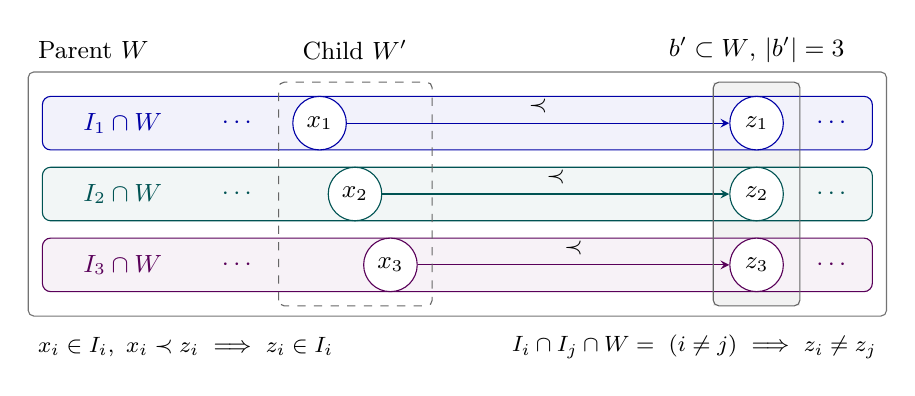
\begin{tikzpicture}[x=1cm,y=1cm,font=\small,>=stealth,
  job/.style={circle,draw,fill=white,minimum size=6.8mm,inner sep=0pt}]
  \draw[black!55,rounded corners=2pt] (-.15,-.25) rectangle (10.75,2.85);
  \node[anchor=west] at (-.15,3.13) {Parent $W$};
  \node at (4,3.13) {Child $W'$};
  \node at (9.1,3.13) {$b'\subset W$, $|b'|=3$};

  \fill[black!5] (8.55,-.12) rectangle (9.65,2.72);
  \foreach \yy/\ii/\xx/\cc in {2.2/1/3.55/blue!65!black,1.3/2/4/teal!65!black,.4/3/4.45/violet!70!black} {
    \draw[draw=\cc,fill=\cc!5,rounded corners=3pt]
      (.03,\yy-.34) rectangle (10.57,\yy+.34);
    \node[text=\cc] at (1.05,\yy) {$I_{\ii}\cap W$};
    \node[text=\cc] at (2.5,\yy) {$\cdots$};
    \node[job,draw=\cc] (x\ii) at (\xx,\yy) {$x_{\ii}$};
    \node[job,draw=\cc] (z\ii) at (9.1,\yy) {$z_{\ii}$};
    \draw[->,draw=\cc] (x\ii) -- node[above,font=\footnotesize] {$\prec$} (z\ii);
    \node[text=\cc] at (10.05,\yy) {$\cdots$};
  }
  \draw[dashed,black!60,rounded corners=2pt] (3.03,-.12) rectangle (4.98,2.72);
  \draw[black!60,rounded corners=2pt] (8.55,-.12) rectangle (9.65,2.72);
  \node[anchor=west,font=\footnotesize] at (-.15,-.64)
    {$x_i\in I_i,\ x_i\prec z_i\ \Longrightarrow\ z_i\in I_i$
     };
  \node[anchor=east,font=\footnotesize] at (10.75,-.64)
    {$I_i\cap I_j\cap W=\varnothing\ (i\ne j)\ \Longrightarrow\ z_i\ne z_j$};
\end{tikzpicture}

\caption{Why at most three injections survive a same-direction update.
For each surviving injection, choose a high job $x_i$ in the child
and a successor $z_i$ in its ending triple $b'$.
Upward closure puts $z_i$ in the same injection; disjointness on the
parent $W$ makes the chosen $z_i$ distinct.
The three-injection case is drawn; arrows denote precedence.
Only witness pairs are shown:
the injections may contain other jobs and may overlap outside $W$.}
\label{fig:capacity-three}
\end{figure}


\subsection{Flattening the history of a run}

Only the first entry of a switch pair can carry a complicated predicate
from an earlier run. The following lemma removes it whenever we need
to reconstruct an old cutoff on a descendant parent.

\begin{lemma}[Local flattening]\label{lem:flatten}
Suppose a run began with a switch out of a node \(Q_0\), using
left boundary \(a_0\) in the resulting run frame, and entries
\[
 G_0\cap\{\rk\ge h_0\},\qquad D_{a_0},
 \qquad Q_0\setminus D_{a_0}\subseteq G_0 .
\]
Let \(U\subseteq Q_0\) be a later parent in that run. If the entry derived from the first displayed entry
survives into an unpruned carry out of \(U\), write its
current form as \(G_0\cap\{\rk\ge k\}\). Then the carried portion
of this pair has the same union on \(U\) as the global upset
\begin{equation}
 D_{a_0}\cup\{\rk\ge k\}.
 \label{eq:flatten}
\end{equation}
\end{lemma}
\begin{proof}
Track the original entries through later reindexings.
As long as the first entry survives, a suffix operation cannot
trim or discard the second entry: a cutoff at that later index
would already discard the first, permanently.
Thus the second entry is either still carried untrimmed, or was
pruned because it was empty on some intermediate node containing
\(U\). In the latter case \(D_{a_0}\cap U=\varnothing\).

On \(U\cap D_{a_0}\), the second entry, when this set is nonempty,
therefore selects every job. Every job of
\(U\setminus D_{a_0}\) lies in \(G_0\), because \(U\subseteq Q_0\).
On that remainder the first entry selects exactly the rank suffix
\(\rk\ge k\). This proves equality of the two unions on \(U\).
Both factors in \eqref{eq:flatten} are upsets, so their union is
globally upward closed, although it need not agree with the
carried pair outside \(U\).
\end{proof}

A new switch out of a node \(W\) uses the edge \(U\to W\)
by which \(W\) was created. Let \(H_-\) be that incoming
edge's low cutoff, in its own working frame, and reserve \(S\)
for the cutoff of the new outgoing edge. We need an extension
of \(H_-\) that does not retain a complicated switch predicate
from an earlier run. Local flattening provides it using lists and
covering properties belonging to already constructed ancestors.

\begin{lemma}[A short extension of an earlier low set]\label{lem:old-low}
Consider an already constructed edge from a parent \(U\) to a child
\(W\), in its old working frame. Its low cutoff \(H_-\subseteq U\)
has a global downset extension \(H_-^*\) agreeing with it on \(U\).
This extension can be chosen with at most \(21\) leaves.
\end{lemma}
\begin{proof}
Use the boundary notation of \(U\) in that old frame for this proof.
If the edge was a switch relative to the tag of \(U\), its low
cutoff is a rank prefix of \(U\setminus D_a\). Thus
\[
 (J\setminus D_a)\cap\{\rk\le r\}
\]
is the required global downset, using at most two leaves.

If the edge was same, its low cutoff on \(U\) equals \(P_b\)
minus its unpruned carry union, without the fresh injection.
The old list on \(U\) has at most five entries by
\Cref{lem:list-length}. If its run began at the root, all carry
entries are simple: the root base or injections, possibly rank-trimmed.
If it began at a switch, the only possibly complicated carry
entry is the first of that switch pair. If it is present in the carry,
replace the carried pair by \eqref{eq:flatten}; if it is absent from
the carry, every carried entry is already simple.

This gives a global upset agreeing with the carry union on \(U\).
It has at most five terms, each with at most four leaves.
Indeed an injection with a rank trim has three leaves; a root
base or a second switch base with a trim has at most two; and
the flattened pair has two. Taking \(P_b\) minus this union
gives a global downset with at most \(1+5\cdot4=21\) leaves.
An empty carry is represented by false.
\end{proof}

\subsection{Constructing the new switch upset}

Suppose a switch out of \(W\) produces a nonempty child.
By \Cref{lem:edge-labels}, \(W\) is not the root.
Let \(U\) be the parent that produced \(W\).
That preceding edge was taken in the tag frame of \(W\), which
is opposite to the current working frame.
In the current frame write \(a_-,b_-\) for the boundaries of \(U\)
and \(v_-\) for its center. The temporal arrangement is
\begin{equation}
 a_-<v_-\le a<b\le b_-.
 \label{eq:ancestry}
\end{equation}
Here \(a\) is an actual ending endpoint of that preceding edge,
viewed in reverse; it can equal \(v_-\).
The node \(W\) lies in the open suffix of \(U\) after \(v_-\);
Figure~\ref{fig:switch} shows this arrangement.

Let \(H_-\) be the low set of the preceding edge in its old
working frame, regarded as a subset of all of \(U\).
The extension \(H_-^*\) from \Cref{lem:old-low} is an upset in
the current, reversed frame. Define
\begin{equation}
 G=D_{a_-}\cap(J\setminus\wP a)
            \cap(J\setminus\wP{v_-})\cap H_-^* .
 \label{eq:G}
\end{equation}

\Needspace{3\baselineskip}
\begin{lemma}\label{lem:G}
The set \(G\) in \eqref{eq:G} is a global upset satisfying both
properties in \eqref{eq:G-properties}.
\end{lemma}
\begin{proof}
All four factors in \eqref{eq:G} are global upsets in the current
frame, so \(G\) is an upset.

Let \(x\in X=W\setminus D_a\).
If \(x\) had been high at the preceding edge in its old frame,
\Cref{lem:edge-labels} would put it in the old predecessor cone
of that edge's ending endpoint. That endpoint is the current \(a\),
so reversal would give \(x\in D_a\), a contradiction.
Thus \(x\in H_-\).
Every job of \(H_-\) precedes the old right boundary of \(U\),
because all edge cutoffs lie in that cone. Equivalently,
\(H_-\subseteq D_{a_-}\) in the current frame.
Since \(x\) is strictly after both \(a\) and \(v_-\), feasibility
excludes \(x\) from their weak predecessor cones.
Finally, \(x\in U\), so agreement of \(H_-^*\) on \(U\) gives
\(x\in H_-^*\). Hence \(X\subseteq G\).

Conversely, suppose \(z\in G\) is scheduled at or before \(a\).
Membership in \(D_{a_-}\), together with \eqref{eq:ancestry},
first places it strictly inside \(U\):
\begin{equation}
 a_-<\operatorname{time}(z)\le a<b\le b_-.
 \label{eq:localize-U}
\end{equation}
Only now use \(H_-^*\cap U=H_-\).
The old edge cutoff \(H_-\) was contained in the old center-low
set. If \(z\) is at or before \(v_-\) in the current frame,
the old center separator puts it in current \(\wP{v_-}\).
If it is strictly after \(v_-\) but at or before \(a\), it lies
in the old normalized side and the old separator at the endpoint
\(a\) puts it in current \(\wP a\).
Both possibilities contradict \eqref{eq:G}.

These separator implications remain valid when preparing the current
node: all intervening reorderings have been confined to \(W=(a,b)\),
and therefore have not changed any job at or before \(a\) in the
current frame, the relevant boundary triples, or the fixed old
cutoff sets.
\end{proof}

\begin{figure}[t]
\centering
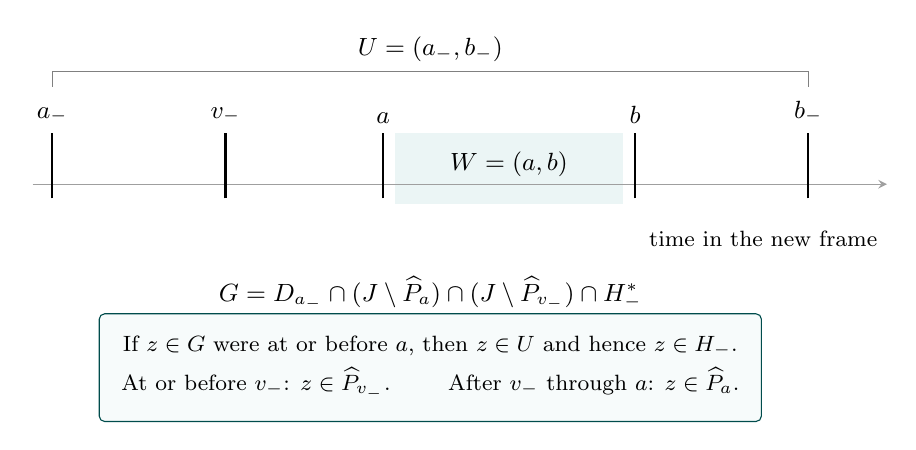
\begin{tikzpicture}[x=1cm,y=1cm,font=\small,>=stealth]
  \fill[teal!8] (4.35,-.25) rectangle (7.25,.65);
  \draw[->,gray!75] (-.25,0) -- (10.6,0);
  \foreach \x in {0,2.2,4.2,7.4,9.6}
    {\draw[thick] (\x,-.18) -- (\x,.65);}
  \node[above] at (0,.65) {$a_-$};
  \node[above] at (2.2,.65) {$v_-$};
  \node[above] at (4.2,.65) {$a$};
  \node[above] at (7.4,.65) {$b$};
  \node[above] at (9.6,.65) {$b_-$};
  \node at (5.8,.25) {$W=(a,b)$};
  \draw[gray] (0,1.24) -- (0,1.43) -- (9.6,1.43) -- (9.6,1.24);
  \node[above] at (4.8,1.43) {$U=(a_-,b_-)$};
  \node[anchor=east,font=\footnotesize] at (10.6,-.7)
    {time in the new frame};
  \node[anchor=north,align=center] at (4.8,-1.05)
    {$G=D_{a_-}\cap (J\setminus\widehat P_a)
      \cap (J\setminus\widehat P_{v_-})\cap H_-^*$};
  \node[draw=teal!60!black,fill=teal!3,rounded corners=2pt,
        inner sep=8pt,align=center,font=\footnotesize] at (4.8,-2.33)
    {If $z\in G$ were at or before $a$, then $z\in U$ and hence $z\in H_-$.\\[3pt]
     At or before $v_-$: $z\in\widehat P_{v_-}$.
     \qquad After $v_-$ through $a$: $z\in\widehat P_a$.};
\end{tikzpicture}

\caption{The ancestor configuration at a direction change, in the new
working frame. A candidate early member of \(G\) is first located
inside \(U\) by \(D_{a_-}\); only there is the earlier cutoff
extension used. The two weak predecessor exclusions then cover
the portions at or before \(v_-\) and between \(v_-\) and \(a\).
The equality \(a=v_-\) is allowed; the intervening segment then
collapses. The horizontal arrow denotes time.}
\label{fig:switch}
\end{figure}

\subsection{Predicate bounds and the induction order}

\begin{lemma}\label{lem:entry-size}
Every entry constructed above has fewer than \(40\) leaves.
This bound persists through any number of same-direction updates.
\end{lemma}
\begin{proof}
Root bases, injections, and second switch bases are simple predicates.
By \Cref{lem:old-low}, the \(H_-^*\) factor in a new \(G\)
has at most \(21\) leaves. The three other factors of \(G\)
and its outer rank suffix use four more. Thus a new first switch
entry has at most \(25\) leaves.
Further same-direction trimming only tightens that outer rank
suffix. It does not append a new independent condition.
The same observation applies to simple entries.
\end{proof}

For completeness, the construction so far has a well-founded
dependency order. Assume the parent and ancestor data already satisfy
their assertions. A same update is defined directly. A switch update
uses the preceding edge's low set; \Cref{lem:old-low} derives its
short extension from already existing lists and, when necessary,
an earlier switch's covering property. \Cref{lem:G} then proves
the new covering and early-exclusion properties.
\Cref{lem:update-labels} supplies the high-set identity and
Invariant~\ref{inv:cones}; \Cref{lem:list-length} supplies the new
length bound; and \Cref{lem:entry-size} supplies the predicate bound.
The length argument needs global closure and high-set identities,
but not the numerical predicate bound. Thus neither bound assumes
itself at a deeper node.

The root starts this induction. We next prove the remaining boundary
invariants for every update, using only the parent invariants and
the current normalizations.
